\documentclass{article}
\usepackage{latexsym}
\usepackage{amssymb,amsmath,amsfonts}
\usepackage{custom2}
\usepackage{graphicx} 
\usepackage{epstopdf} 
\usepackage{caption}
\usepackage{subcaption}
\usepackage{url}
\usepackage[all,arc]{xy}
\usepackage{enumerate}
\usepackage{mathrsfs}
\usepackage{booktabs}
\usepackage[pdftex]{hyperref}
\usepackage{lscape}
\usepackage{xcolor}
\usepackage{natbib}
\usepackage{tabularx}
\newcommand{\tabitem}{~~\llap{\textbullet}~~}

\captionsetup{justification=RaggedRight, singlelinecheck=false}
\newcommand{\ra}[1]{\renewcommand{\arraystretch}{#1}}
\newcommand{\argmax}{\text{argmax}}
\newcommand{\Tr}{\text{Tr}}
\newcommand{\mb}{\mathbf}
\newtheorem{ass}{Assumption}

\addtolength{\evensidemargin}{-.5in}
\addtolength{\oddsidemargin}{-.5in}
\addtolength{\textwidth}{1.4in}
\addtolength{\textheight}{1.4in}
\addtolength{\topmargin}{-.5in}

\pagestyle{empty}

\title{Conflict and Strategy in Collective Computation}
\author{Eleanor Brush, David Krakauer, Jessica Flack}

\begin{document}
\maketitle
\tableofcontents

%\appendix
\section*{Supplementary Information}
\renewcommand{\thesubsection}{\Alph{subsection}.}
\renewcommand{\thesubsubsection}{\thesubsection \arabic{subsubsection}}
%\renewcommand{\thetheorem}{\thesubsection .\arabic{theorem}}
\renewcommand{\thetheorem}{\arabic{theorem}}

\subsection{Derivation of PDEs for waiting time and accuracy \label{pdes_deriv}}
\subsubsection{SDEs }
%(Section 4.3.6 Stochastic Differential Equations, Multivariable Systems in Gardiner) 
In the following we will assume we have a set of stochastic differential equation written as
\begin{equation}
d{\mathbf x} ={\mb A}({\mb x},t)dt+{\mb B}({\mb x},t)d{\mb W}(t), \label{sde}
\end{equation}
where ${\mb x}\in\R^N$, $A:\R^N\times \R\to\R^N$, ${\mb B}:\R^N\times\R\to\R^N\times\R^N$, and $d{\mb W}(t)$ is an $N$ variable Weiner process. The forward equation describing the probability density $p({\mb x},t|{\mb y},s)$ is 
%% i'm trying to be consistent about my noise terms: I'll try to always use B*B^T even though Gardiner seems to switch back and forth between B and B*^T
\begin{equation}
\frac{\partial p}{\partial t} =-\sum_{i=1}^N\frac{\partial \big(A_i({\mb x},t)p\big)}{\partial x_i}+\frac{1}{2}\sum_{i,j=1}^N\frac{\partial^2\big([{\mb B}({\mb x},t){\mb B}^T({\mb x},t)]_{ij}p\big)}{\partial x_i\partial x_j} \label{forward}
\end{equation}
and the backward equation is 
\begin{equation}
-\frac{\partial p}{\partial s}=\sum_{i=1}^NA_i({\mb y},s)\frac{\partial p}{\partial y_i}+\frac{1}{2}\sum_{i,j=1}^N[{\mb B}({\mb y},s){\mb B}^T({\mb y},s)]_{ij}\frac{\partial^2 p}{\partial y_i\partial y_j}. \label{backward}
\end{equation}

\subsubsection{Expected first exit time }
%(section 5.5 the Fokker-Planck Equation, First Passage Times for Homogeneous Processes in Gardiner) 
Let $G({\mathbf y},t)$ be the probability that the particle is still in the region $R$ at time $t$ given that it started at ${\mathbf y}$ so that $$G({\mathbf y},t)=\int_Rp({\mathbf x},t|{\mathbf y},0)d{\mathbf x}.$$  

\begin{claim} If the system is time homogeneous,
\begin{equation}
\frac{\partial G}{\partial t}=\sum_{i=1}^NA_i({\mb y})\frac{\partial G}{\partial y_i}+\frac{1}{2}\sum_{i,j=1}^N[{\mb B}({\mb y}){\mb B}^T({\mb y})]_{ij}\frac{\partial^2 G}{\partial y_i\partial y_j}. \label{Geq}
\end{equation}
%%Gardiner has a 2 instead of 1/2 in Section 6.6 but that must be a typo
\end{claim}
\begin{pf}
If the system is time homogeneous, then $p({\mb x},t|{\mb y},0)=p({\mb x},0|{\mb y},-t)$ so that we can rewrite $G$ as 
\begin{align*}
G({\mb y},t)&=\int_Rp({\mb x},0|{\mb y},-t)d{\mb x},
\\ \text{ which gives that } \frac{\partial G}{\partial t}\bigg|_{t=t}&=\int_R\frac{\partial p({\mb x},0|{\mb y},-t)}{\partial t}\bigg|_{t=t}d{\mb x}
\\&=\int_R -\frac{\partial p({\mb x},0|{\mb y},s)}{\partial s}\bigg|_{s=t} d{\mb x}
\\&=\int_R\bigg(\sum_{i=1}^NA_i({\mb y})\frac{\partial p}{\partial y_{i}}\bigg|_{s=t}+\frac{1}{2}\sum_{i,j=1}^N[{\mb B}({\mb y}){\mb B}^T({\mb y})]_{ij}\frac{\partial^2 p}{\partial y_{i}\partial y_{j}}\bigg|_{s=t}\bigg) d{\mb x} \text{ using (\ref{backward})}
\\&=\sum_{i=1}^NA_i({\mb y})\bigg(\int_R\frac{\partial p}{\partial y_{i}}\bigg|_{s=t}d{\mb x}\bigg)+\frac{1}{2}\sum_{i,j=1}^N[{\mb B}({\mb y}){\mb B}^T({\mb y})]_{ij}\bigg(\int_R\frac{\partial^2 p}{\partial y_{i}\partial y_{j}}\bigg|_{s=t}\bigg) d{\mb x}
\\&=\sum_{i=1}^NA_i({\mb y})\frac{\partial G}{\partial y_i}+\frac{1}{2}\sum_{i,j=1}^N[{\mb B}({\mb y}){\mb B}^T({\mb y})]_{ij}\frac{\partial^2 G}{\partial y_i\partial y_j}
\end{align*}
\end{pf}

We can now use Equation (\ref{Geq}) to find an equation that the expected hitting time satisfies. If $T$ is the time at which the particle hits the boundary $S=\partial R$, then $P(T\geq t|{\mb y})=G({\mathbf y},t)$.  Therefore
\begin{align*}
E_{{\mathbf y}}(T) &=\int_0^\infty t P(T\in[t,t+dt)|{\mathbf y})
\\&= \int_0^\infty t \bigg(P(T\geq t|{\mathbf y})-P(T\geq t+dt|{\mathbf y})\bigg) 
\\&=\int_0^\infty t \bigg(G({\mathbf y},t)-G({\mathbf y},t+dt)\bigg)
\\&=\int_0^\infty t \frac{G({\mathbf y},t)-G({\mathbf y},t+dt)}{dt}dt
\\&=-\int_0^\infty t\frac{\partial G}{\partial t}dt
\\&=-\bigg(\big[tG({\mathbf y},t)\big]_0^{\infty}-\int_0^\infty G({\mathbf y},t)dt\bigg)  \text{ by integration by parts }
\\&=\int_0^\infty G({\mathbf y},t)dt \text{ if $\lim_{t\to \infty}G({\mathbf y},t)=0$ quickly enough}.
\end{align*}

If we let $f({\mathbf y})=E_{\mathbf y}(T)$, then 
\begin{align*}
\sum_{i=1}^NA_i({\mb y},t)\frac{\partial f}{\partial y_i}+\frac{1}{2}\sum_{i,j=1}^N[{\mb B}({\mb y},t){\mb B}^T({\mb y},t)]_{ij}\frac{\partial^2 f}{\partial y_i\partial y_j}&=\int_0^\infty\bigg(\sum_{i=1}^NA_i({\mb y},t)\frac{\partial G}{\partial y_i}+\frac{1}{2}\sum_{i,j=1}^N[{\mb B}({\mb y},t){\mb B}^T({\mb y},t)]_{ij}\frac{\partial^2 G}{\partial y_i\partial y_j}\bigg)dt
\\&=\int_0^\infty\frac{\partial G}{\partial t}dt \text{ using (\ref{Geq})}
\\&=G({\mb y},\infty)-G({\mb y},0)
\\&=-1
\end{align*}
Finally, this gives us a PDE for the expected hitting time of the boundary of the region $R$:
\begin{equation}
\sum_{i=1}^NA_i({\mb y})\frac{\partial f}{\partial y_i}+\frac{1}{2}\sum_{i,j=1}^N[{\mb B}({\mb y}){\mb B}^T({\mb y})]_{ij}\frac{\partial^2 f}{\partial y_i\partial y_j}=-1 \label{DT}
\end{equation}
with boundary conditions $f({\mb x})=0 \text{ for } {\mb x}\in\partial R$.

\subsubsection{Distribution of exit points }
%(section 6.6.2 The Fokker-Planck Equation in Several Dimensions, Distribution of Exit Points and section 5.5.4 Probability of Exit Through a Particular End of the Interval in Gardiner )
Let ${\mb J}({\mb x},t|{\mb y},s):(\R^N\times\R)\times(\R^N\times\R)\to \R^N$ be such that 
$$J_k({\mb x},t|{\mb y},s)=A_k({\mb x},t)p({\mb x},t|{\mb y},s)-\frac{1}{2}\sum_{l=1}^N\frac{\partial \big([{\mb B}({\mb x},t){\mb B}^T({\mb x},t)]_{kl}p({\mb x},t|{\mb y},s)\big)}{\partial x_j}.$$ 
If $p$ satisfies the forward equation (\ref{forward}), then 
\begin{equation}
\frac{\partial p}{\partial t} =-\sum_{i=1}^N\frac{\partial \big(A_i({\mb x},t)p\big)}{\partial x_i}+\frac{1}{2}\sum_{i,j=1}^N\frac{\partial^2\big([{\mb B}({\mb x},t){\mb B}^T({\mb x},t)]_{ij}p\big)}{\partial x_i\partial x_j}=-\sum_{i=1}^N\frac{\partial J_i({\mb x},t|{\mb y},s)}{\partial x_i}. \label{jequals}
\end{equation}

\begin{claim}
Each $J_k$  satisfies the backward equation.
\end{claim}
\begin{pf}
{\tiny
\begin{align*}
\sum_{i=1}^NA_i({\mb y},s)\frac{\partial J_k({\mb x},t|{\mb y},s)}{\partial y_i}+\frac{1}{2}\sum_{i,j=1}^N[{\mb B}({\mb y},s){\mb B}^T({\mb y},s)]_{ij}\frac{\partial^2 J_k({\mb x},t|{\mb y},s)}{\partial y_i\partial y_j}
&=\sum_{i=1}^NA_i({\mb y},s)\bigg[A_k({\mb x},t)\frac{\partial p}{\partial y_i}-\frac{1}{2}\sum_{l=1}^N\frac{\partial \bigg([{\mb B}({\mb x},t){\mb B}^T({\mb x},t)]_{kl}\frac{\partial p({\mb x},t|{\mb y},s)}{\partial y_i}\bigg)}{\partial x_l}\bigg]
\\&+\frac{1}{2}\sum_{i,j=1}^N[{\mb B}({\mb y},s){\mb B}^T({\mb y},s)]_{ij}\bigg[A_k({\mb x},t)\frac{\partial^2 p}{\partial y_i\partial y_j}-\frac{1}{2}\sum_{l=1}^N\frac{\partial \bigg([{\mb B}({\mb x},t){\mb B}^T({\mb x},t)]_{kl}\frac{\partial^2 p({\mb x},t|{\mb y},s)}{\partial y_iy_j}\bigg)}{\partial x_l}\bigg]
\\&=A_k({\mb x},t)\bigg[\sum_{i=1}^NA_i({\mb y},s)\frac{\partial p}{\partial y_i}+\frac{1}{2}\sum_{i,j=1}^N[{\mb B}({\mb y},s){\mb B}^T({\mb y},s)]_{ij}\frac{\partial^2 p}{\partial y_i\partial y_j}\bigg]
\\&-\frac{1}{2}\sum_{l=1}^N\frac{\partial }{\partial x_l}\bigg([{\mb B}({\mb x},t){\mb B}^T({\mb x},t)]_{kl}\bigg[\sum_{i=1}^NA_i({\mb y},s)\frac{\partial p}{\partial y_i}+\frac{1}{2}\sum_{i,j=1}^N[{\mb B}({\mb y},s){\mb B}^T({\mb y},s)]_{ij}\frac{\partial^2 p}{\partial y_i\partial y_j}\bigg)\bigg]
\\&=A_k({\mb x},t)\bigg(-\frac{\partial p}{\partial s}\bigg)-\frac{1}{2}\sum_{l=1}^N\frac{\partial }{\partial x_l}\bigg(-[{\mb B}({\mb x},t){\mb B}^T({\mb x},t)]_{kl}\frac{\partial p}{\partial s}\bigg) \text{ using (\ref{backward})}
\\&=-\frac{\partial }{\partial s}\bigg(A_k({\mb x},t)p({\mb x},t|{\mb y},s)-\frac{1}{2}\sum_{l=1}^N\frac{\partial \big([{\mb B}({\mb x},t){\mb B}^T({\mb x},t)]_{kl}p({\mb x},t|{\mb y},s)\big)}{\partial x_l}\bigg)
\\&=-\frac{\partial J_k}{\partial s}.
\end{align*}
}
\end{pf}


It follows that any linear combination $q({\mb x},t|{\mb y},s)=\sum_{k=1}^Nc_kJ_k({\mb x},t|{\mb y},s)$ also satisfies the backward equation:
\begin{equation}
-\frac{\partial q}{\partial s}=\sum_{i=1}^NA_i({\mb y},s)\frac{\partial q}{\partial y_i}+\frac{1}{2}\sum_{i,j=1}^N[{\mb B}({\mb y},s){\mb B}^T({\mb y},s)]_{ij}\frac{\partial ^2 q}{\partial y_i\partial y_j}. \label{jbackeq}
\end{equation}

\begin{claim} \label{probcurrent}
If $S_{12}$ represents the boundary between two regions $R_2$ and $R_2$, then the net flow of probability from $R_2$ to $R_1$ can be written as $\int_{S_{12}} dS {\mb n}\cdot {\mb J}({\mb x},t) $ where ${\mb n}$ is a normal vector from $R_2$ to $R_1$.  
\end{claim}

\begin{pf}
Let $S_1$ be the part of the boundary of $R_1$ not shared with $R_2$ and $S_2$ be the part of the boundary of $R_2$ not shared with $R_1$ so that  $\partial R_1=S_1\cup S_{12}$, $R_2=S_2\cup S_{12}$, and $S_1\cap S_{12}=S_2\cap S_{12}=\emptyset$. The probability of crossing from $R_2$ to $R_1$ across $S_{12}$ in the interval of time $[t,t+dt)$ is 
\begin{align*}
\int_{R_1}d{\mb x}\int_{R_2}d{\mb y} p({\mb x},t+dt|{\mb y},t).
\end{align*}



The probability of crossing from $R_1$ to $R_2$ across $S_{12}$  in the interval of time $[t,t+dt)$ can be found analogously so the net flow $F$ from $R_2$ to $R_1$ at time $t$ is 
\begin{align*}
F=\lim_{dt \to 0}\frac{1}{dt}\int_{R_1}d{\mb x}\int_{R_2}d{\mb y} \big(p({\mb x},t+dt|{\mb y},t)-p({\mb y},t+dt|{\mb x},t)\big).
\end{align*}
Since $p({\mb x},t|{\mb y},t)=p({\mb y},t|{\mb x},t)=0$ for ${\mb y}\in R_2$ and ${\mb x}\in R_1$,
\begin{align*}
F&=\lim_{dt \to 0}\frac{1}{dt}\int_{R_1}d{\mb x}\int_{R_2}d{\mb y} \big(p({\mb x},t+dt|{\mb y},t)-p({\mb x},t|{\mb y},t)-p({\mb y},t+dt|{\mb x},t)+p({\mb y},t|{\mb x},t)\big)
\\&=\int_{R_1}d{\mb x}\int_{R_2}d{\mb y} \bigg(\frac{\partial p({\mb x},t'|{\mb y},t)}{\partial t'}\bigg|_{t'=t}-\frac{\partial p({\mb y},t'|{\mb x},t)}{\partial t'}\bigg|_{t'=t}\bigg)
\\&=\int_{R_1}d{\mb x}\int_{R_2}d{\mb y}\bigg(-\sum_{i=1}^N\frac{\partial J_i({\mb x},t|{\mb y},t)}{\partial x_i}+\sum_{i=1}^N\frac{\partial J_i({\mb y},t|{\mb x},t)}{\partial y_i}\bigg) \text{using (\ref{jequals})}
\\&=\int_{R_1}d{\mb x}\int_{R_2}d{\mb y}\sum_{i=1}^N\frac{\partial J_i({\mb y},t|{\mb x},t)}{\partial y_i}-\int_{R_2}d{\mb y}\int_{R_1}d{\mb x}\sum_{i=1}^N\frac{\partial J_i({\mb x},t|{\mb y},t)}{\partial x_i}
\\&=\int_{R_1}d{\mb x}\bigg[\int_{S_2}dS {\mb n_2}\cdot {\mb J}({\mb y},t|{\mb x},t)+\int_{S_{12}}dS {\mb n_2}\cdot {\mb J}({\mb y},t|{\mb x},t)\bigg]-\int_{R_2}d{\mb y}\bigg[\int_{S_1}dS{\mb n}_1\cdot{\mb J}({\mb x},t|{\mb y},t)+\int_{S_{12}}dS{\mb n}_1\cdot{\mb J}({\mb x},t|{\mb y},t)\bigg]
\\ &\text{ where ${\mb n}_2$ is a normal pointing out of $R_2$ and similarly for ${\mb n}_1$, by the divergence theorem}
\end{align*}
For ${\mb y}\in S_2$ and ${\mb x}\in R_1$, $J({\mb y},t|{\mb x},t)=0$. Similarly, for ${\mb x}\in S_1$ and ${\mb y}\in R_2$, ${\mb J}({\mb x},t|{\mb y},t)=0$.  Therefore, the integrals over $S_2$ and $S_1$ disappear and $F$ simplifies to
\begin{align*}
F&=\int_{R_1}d{\mb x}\bigg[\int_{S_{12}}dS {\mb n_2}\cdot {\mb J}({\mb y},t|{\mb x},t)\bigg]-\int_{R_2}d{\mb y}\bigg[\int_{S_{12}}dS{\mb n}_1\cdot{\mb J}({\mb x},t|{\mb y},t)\bigg]
\\&=\int_{S_{12}}dS\bigg[\int_{R_1}d{\mb y}\ {\mb n}\cdot \mb{J}({\mb x},t|{\mb y},t)+\int_{R_2}d{\mb y}\ {\mb n}\cdot {\mb J}({\mb x},t|{\mb y},t)\bigg]
\\ & \text{ where ${\mb n}$ is a normal pointing from $R_2$ to $R_1$}
\\&=\int_{S_{12}}dS\bigg[\int_{R_1\cup R_2}d{\mb y}\ {\mb n}\cdot \mb{J}({\mb x},t|{\mb y},t)\bigg]
\\&=\int_{S_{12}}dS\ {\mb n}\cdot {\mb J}({\mb x},t) \text{ since ${\mb x}\in S_{12}\subset R_1\cup R_2$}
\end{align*}
\end{pf}

Now consider a region $R$ with boundary $S$.  Let $g({\mb a},{\mb x},t)|d{\mb S}({\mb a})|$ be the probability of exiting through an element $d{\mb S}({\mb a})$ of the boundary $S$ after time $t$.

\begin{claim}
If the system is time homogeneous, 
\begin{equation}
\frac{\partial g}{\partial t}=\sum_{i=1}^NA_i({\mb x})\frac{\partial g}{\partial x_i}+\frac{1}{2}\sum_{i,j=1}^N[{\mb B}({\mb x}){\mb B}^T({\mb x})]_{ij}\frac{\partial ^2 g}{\partial x_i\partial x_j}. \label{geq}
\end{equation}
\end{claim}

\begin{pf}
By the definition of $g$,
{\tiny
%% Gardiner has a negative sign in the following but I don't know why and it seems to work out just fine without it?
\begin{align*}
g({\mb a},{\mb x},t)|d{\mb S}({\mb a})|&=\int_t^\infty dt' {\mb J}({\mb a},t'|{\mb x},0)\cdot d{\mb S}(\mb{a}) \text{using Claim \ref{probcurrent}}
\\&=\int_t^\infty dt' {\mb J}({\mb a},0|{\mb x},-t')\cdot d{\mb S}(\mb{a})
\\&=\int_{-\infty}^{-t}dt' {\mb J}({\mb a},0|{\mb x},t')\cdot d{\mb S}(\mb{a}) \text{ using integration by substitution}
\\ \text{ so that }  \sum_{i=1}^NA_i({\mb x})\frac{\partial g}{\partial x_i}+\frac{1}{2}\sum_{i,j=1}^N[{\mb B}({\mb x}){\mb B}^T({\mb x})]_{ij}\frac{\partial ^2 g}{\partial x_i\partial x_j}
&=\int_{-\infty}^{-t} dt'\bigg(\sum_{i=1}^NA_i({\mb x})\frac{\partial ({\mb J}({\mb a},0|{\mb x},t')\cdot d{\mb S}({\mb a}))}{\partial x_i}+\frac{1}{2}\sum_{i,j=1}^N[{\mb B}({\mb x}){\mb B}^T({\mb x})]_{ij}\frac{\partial ^2 ({\mb J}({\mb a},0|{\mb x},t')\cdot d{\mb S}({\mb a}))}{\partial x_i\partial x_j}\bigg)
\\&=\int_{-\infty}^{-t}dt' \bigg(-\frac{\partial ({\mb J}({\mb a},0|{\mb x},t')\cdot d{\mb S}({\mb a}))}{\partial t'}\bigg) \text{ using (\ref{jbackeq})}
\\&=\big(-{\mb J}({\mb a},0|{\mb x},t')\cdot d{\mb S}({\mb a})\big)\bigg|_{-\infty}^{-t}
\\&=\big(-{\mb J}({\mb a},-t'|{\mb x},0)\cdot d{\mb S}({\mb a})\big)\bigg|_{-\infty}^{-t}
\\&=-{\mb J}({\mb a},t|{\mb x},0)\cdot d{\mb S}({\mb a})\
\\&=\frac{\partial g}{\partial t}
\end{align*}
}
\end{pf}

We are interested in finding the total probability of exiting through $d{\mb S}({\mb a})$, $h({\mb a},{\mb x})=g({\mb a},{\mb x},0)$.  If we let $t\to 0$ in (\ref{geq}) and notice that ${\mb J}({\mb a},0|{\mb x},0)=\delta(|{\mb a}-{\mb x}|)$, we find that 
\begin{equation*}
\sum_{i=1}^NA_i({\mb x})\frac{\partial h}{\partial x_i}+\frac{1}{2}\sum_{i,j=1}^N[{\mb B}({\mb x}){\mb B}^T({\mb x})]_{ij}\frac{\partial ^2 h}{\partial x_i\partial x_j}=0
\end{equation*}
with boundary conditions $h({\mb a},{\mb x})=\delta(|{\mb a}-{\mb x}|)$ for ${\mb x}$ in $S$. To find the total probability of exiting through a section $S'\subset S$, $H(S',{\mb x})$ we can simply integrate the solutions $h({\mb a},{\mb x})$ for ${\mb a}\in S'$ to find 
\begin{equation}
\sum_{i=1}^NA_i({\mb x})\frac{\partial H}{\partial x_i}+\frac{1}{2}\sum_{i,j=1}^N[{\mb B}({\mb x}){\mb B}^T({\mb x})]_{ij}\frac{\partial ^2 H}{\partial x_i\partial x_j}=0 \label{ER}
\end{equation}
with boundary conditions $H(S',{\mb x})=\delta({\mb x}\in S')$ for ${\mb x}\in S$.

We will introduce the operator ${\mb L}$ such that 
\begin{equation}
{\mb L}(f)=\sum_{i=1}^NA_i({\mb x})\frac{\partial f}{\partial x_i}+\frac{1}{2}\sum_{i,j=1}^N[{\mb B}({\mb x}){\mb B}^T({\mb x})]_{ij}\frac{\partial ^2 f}{\partial x_i\partial x_j}. \label{operator}
\end{equation}
Then the expected time to hit the boundary $S$ satisfies ${\mb L}f=-1$ with boundary conditions $f({\mb x})=0$ for ${\mb x}\in S$ and the probability of hitting a subset $S'\subset S$ satisfies ${\mb L}H=0$ with boundary conditions $H({\mb x})=\delta({\mb x}\in S')$ for ${\mb x}\in S$.

%We can also consider the expected exit time, given that the particle exits through $d{\mb S}({\mb a})$, $T({\mb a},{\mb x})$:
%
%\begin{align*}
%T({\mb a},{\mb x})&=\int_0^\infty t P(\text{ exit in }[t,t+dt)|\text{ exit through }d{\mb S}({\mb a}))
%\\&=\int_0^\infty t\frac{P(\text{ exit through }d{\mb S}({\mb a}) \text{ in }[t,t+dt))}{P(\text{ exit through } d{\mb S}({\mb a}))}
%\\&=\frac{1}{{P(\text{ exit through } d{\mb S}({\mb a}))}}\int_0^\infty t P(\text{ exit through }d{\mb S}({\mb a}) \text{ in }[t,t+dt))
%\\&=\frac{1}{h({\mb a},{\mb x})}\int_0^\infty t\bigg(g({\mb a},{\mb x},t)-g({\mb a},{\mb x},t+dt)\bigg)
%\\&=\frac{1}{h({\mb a},{\mb x})}\int_0^\infty- t\frac{\partial g}{\partial t}dt
%\\&=-\frac{1}{h({\mb a},{\mb x})}\bigg([tg({\mb a},{\mb x},t)]_0^\infty-\int_0^\infty g({\mb a},{\mb x},t)dt\bigg) \text{ by integration by parts}
%\\&=\frac{1}{h({\mb a},{\mb x})}\int_0^\infty g({\mb a},{\mb x},t)dt \text{ if }\lim_{t\to\infty} g({\mb a},{\mb x},t)=0 \text{ quickly enough}
%\\\text{so that }T({\mb a},{\mb x})h({\mb a},{\mb x})&=\int_0^\infty g({\mb a},{\mb x},t)dt
%\end{align*}
%If we integrate (\ref{geq}) from $0$ to $\infty$ we find that 
%\begin{align*}
%-h({\mb a},{\mb x})=-g({\mb a},{\mb x},0)=\sum_{i=1}^NA_i({\mb x})\frac{\partial (Th)}{\partial x_i}+\frac{1}{2}\sum_{i,j=1}^N[{\mb B}({\mb x}){\mb B}^T({\mb x})]_{ij}\frac{\partial^2(Th)}{\partial x_i\partial x_j}.
%\end{align*}


\subsubsection{Our model }
The stochastic differential equations in our model are
\begin{equation}
\begin{array}{ll}
dX_1&=\bigg(-\ell X_1(t)+br(2c-1)\bigg)dt+\bigg(b\sqrt{rc}\bigg)dW_\text{L}t-\bigg(b\sqrt{r(1-c)}\bigg)dW_\text{R}t
\\dX_2&=\bigg(-\ell X_2(t)-br(2c-1)\bigg)dt-\bigg(b\sqrt{rc}\bigg)dW_\text{L}t+\bigg(b\sqrt{r(1-c)}\bigg)dW_\text{R}t.
\end{array}
\end{equation}

This gives 
\begin{equation}
{\mb A}({\mb x},t)=\left(\begin{array}{ll} 
-\ell x_1+br(2c-1)
\\ -\ell x_2-br(2c-1)
\end{array}\right), \text{ and }
\end{equation}

\begin{equation}
{\mb B}({\mb x},t)=\left(\begin{array}{ll} 
b\sqrt{rc} & -b\sqrt{r(1-c)}
\\ -b\sqrt{rc} & b\sqrt{r(1-c)}
\end{array}\right), \text{ so that }
\end{equation}

\begin{equation}
{\mb B}({\mb x},t){\mb B}^T({\mb x},t)
=\left(\begin{array}{ll}
b^2r & b^2r
\\ b^2r & b^2r
\end{array}\right)
\end{equation}

Thus, the operator ${\mb L}$ is given by

\begin{align}
%\begin{array}{ll}
{\mb L}(f)&=(-\ell x_1+br(2c-1))\frac{\partial f}{\partial x_1}+(-\ell x_2-br(2c-1))\frac{\partial f}{\partial x_2}+\frac{1}{2}b^2r\frac{\partial^2 f}{\partial x_1^2}+\frac{1}{2}b^2r\frac{\partial^2 f}{\partial x_1\partial x_2}+\frac{1}{2}b^2r\frac{\partial^2 f}{\partial x_2\partial x_1}+\frac{1}{2}b^2r\frac{\partial^2 f}{\partial x_2^2} \notag
\\&=(-\ell x_1+br(2c-1))\frac{\partial f}{\partial x_1}+(-\ell x_2-br(2c-1))\frac{\partial f}{\partial x_2}+b^2r\bigg(\frac{1}{2}\frac{\partial^2 f}{\partial x_1^2}+\frac{\partial^2 f}{\partial x_1\partial x_2}+\frac{1}{2}\frac{\partial^2 f}{\partial x_2^2} \bigg)
%\end{array}
\end{align}

The region we are interested in is the one in which both individuals' opinions $(x_1,x_2)$ are greater than or equal to their respective thresholds, i.e. $R=\{(x_1,x_2): x_1\geq -T_1 \text{ and } x_2\geq -T_2\}$ so that $S=\partial R=\{(x_1,-T_2): x_1>-T_1\}\cup\{(-T_1,x_2):x_2>-T_2\}$.  The subset of the boundary we are interested in is the one that indicates a correct decision has been made, i.e. $x_2=-T_2$, so that $S'=\{(x_1,-T_2):x_1>-T_1\}$. The expected decision time is the expected hitting time of $S$ and the probability of a correct decision is the probability that the exit is through $S'$. 

In order to  numerically solve the PDEs for decision time and error rate, we artificially close the region $R$ so that we can impose boundary conditions on a finite subset of the plane. In order to this, we pick two upper bounds $B_1$ and $B_2$ and restrict $R$ to $$R_2=\{(x_1,x_2): x_1\in [-T_1,B_1] \text{ and } x_2\in[ -T_2,B_2]\},$$ with boundary $S_2$. The subset of the boundary we are interested in becomes 
$$S'_2=\{(x_1,-T_2):x_1\in [-T_1,B_1]\}\cup\{(B_1,x_2):x_2\in [-T_2,B_2]\}$$
The boundary condition $f({\mb x})=0$ for ${\mb x}\in S$ becomes $f({\mb x})=0$ for ${\mb x}\in S_2$ and the condition $H({\mb x})=\delta({\mb x}\in S')$ for ${\mb x}\in S$ becomes $H({\mb x})=\delta({\mb x}\in S'_2)$ for ${\mb x}\in S_2$.

\subsection{Initial conditions } 

\subsection{Analysis of homogeneous abilities }

\subsection{Explanation for most informative measures }

Which measure is the most informative about the individuals' true values depends on how accurately pairwise decisions tend to be and what kind of errors are most frequent. When decisions are quite accurate ($w_2<.4$), the finer measures of consensus---weighted in-degree and eigenvector centrality---can use all of the information in the decision network to make fine distinctions between individuals, leading to consensus scores that are more informative than those from the coarser measures---in-degree and entropy.  Whether weighted in-degree or eigenvector centrality is more informative depends on what type of error is common. When there are no waiting costs ($w_2=0$) and the individuals value their personal preferences over accuracy ($w_1<.8$), low valued individuals can sometimes wait out higher valued individuals leading to an incorrect  decision being made in favor of a low individual at the expense of a high individual. Since eigenvector centrality takes the identity of the source of decisions into account, it will incorrectly assign the low individual a high score, whereas weighted in-degree will ignore the source and assign the low individual an appropriately low score.  Therefore, in these circumstances, weighted in-degree is more informative. When accuracy matters ($w_1\geq .8$, $w_2=0$) or when there are low non-zero waiting costs ($0<w_2\leq .3$) low value individual are less likely to wait out high value individuals, but there are a moderate amount of mistakes between pairs of individuals in the middle and bottom of the group. Consider two middle value individuals, with $A$ having slightly higher value than $B$. Another individual might make a mistake with respect to $B$ so that weighted in-degree gives $B$ a slightly higher score than $A$. But $A$ and $B$ will tend to decide correctly so that, despite errors, $B$ will send more decisions than $A$. Since eigenvector centrality is affected by the decisions sent as well as received, it will correctly give $A$ a higher score. Therefore, in these circumstances, eigenvector centrality is the most informative. As waiting costs increase ($.4 \leq w_2 \leq .5$) and decisions become even less accurate, even the high value individuals start to make mistakes. Now consider two high value individuals, with $A$ having slight higher value than $B$. If $A$ errs and decides strongly in favor of a lower value individual, eigenvector centrality will give $A$ a lower score because of those sent decisions and weighted in-degree will give $A$ a lower score because of the decisions it has prevented itself from receiving. However, $A$ is likely to make at most one more mistake than $B$ so that the number of individuals deciding in favor of either will be the same. Thus the coarseness of unweighted in-degree becomes an advantage by allowing it to group high value individuals together when finer measures would make incorrect fine distinctions. When decisions are even less accurate ($.5<w_2<.7$), weighted in-degree, unweighted in-degree, and eigenvector centrality can all get confused by incorrect decisions between any pair of individuals. What becomes especially difficult is distinguishing between low value individuals, one of whom might incorrectly receive decisions from higher individuals. If a low value individual receives correct decisions, they will be of similar strengths from even lower individuals. However, if it receives decisions from a higher individual, even though its score from any of the other measures will be increased, entropy decreases its score because of the difference in the strengths of signals coming from different types of individuals. In these circumstances, entropy does well at measuring the lack of consensus of decisions with respect of low individuals. When decisions are very inaccurate ($w_2>.6$), weighted in-degree becomes the most reliable.
 




\subsection{Supplemental Figures }

\renewcommand{\thefigure}{S\arabic{figure}}
\setcounter{figure}{0}  

\begin{figure}[ht]
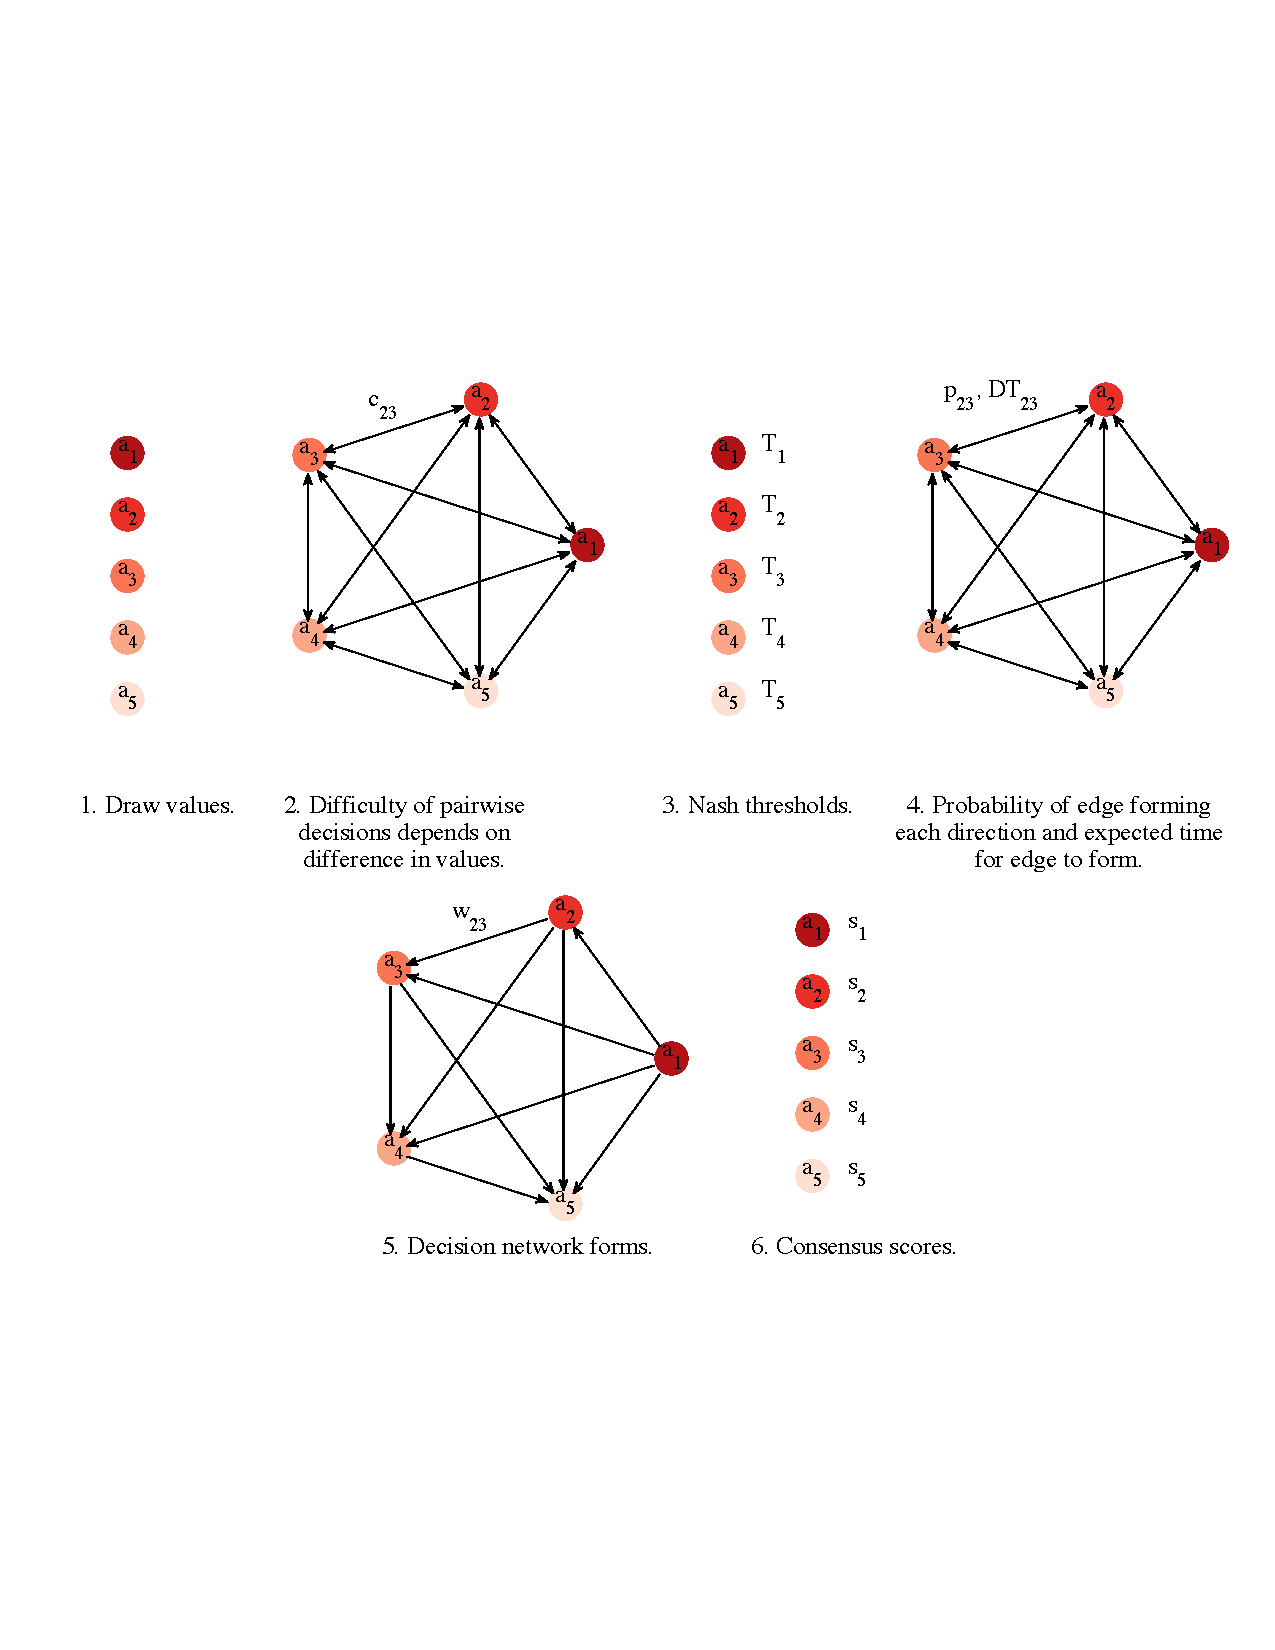
\includegraphics[width=6.83in]{cartoon_cropped.pdf}
\caption{\label{cartoon} Schematic of the development of the decision network. 1. First, each individual's value is drawn from a uniform distribution. 2. The difficulty of each pairwise decision increases with the similarity of values, so that $c_{ij}$ increases as $|a_i-a_j|$ increases. 3. Given these difficulties, each individual has a Nash threshold strategy $T_i$. 4. Given the set of Nash thresholds, a pair will reach each decision with some probability and in an expected amount of time. 5. We draw the decisions according to the probabilities of the two possible outcomes and the strength of the decision decreases with increasing decision time. 6. For each decision network, we compute a set of consensus measures to give each individual a consensus score. We repeat this process for many random draws of values to find average Nash thresholds and the mutual information between the consensus scores and the values. }
\end{figure}

\begin{figure}[ht]
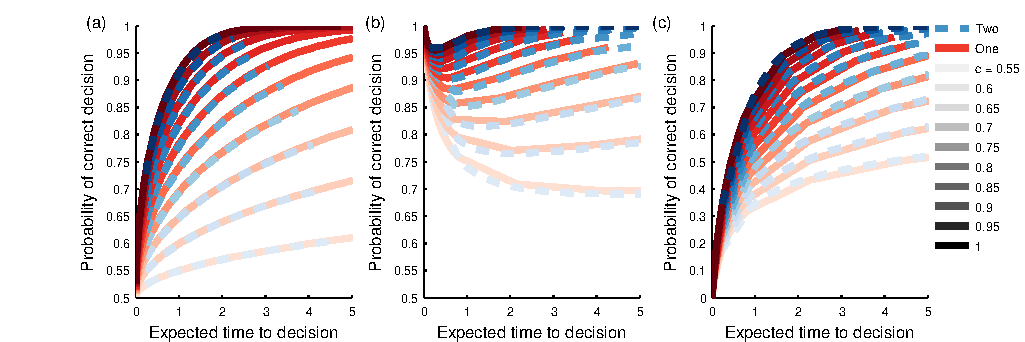
\includegraphics[width=\textwidth]{dimensionality_comparison.pdf}
\caption{\label{dimensionality} The accuracy of decision-making is the same for the reduced one-dimensional model and the full two-dimensional model. In each version of the model, changing the decision thresholds changes the probability of a correct decision and the expected time to a decision. Here we show the probability of a correct output as a function of the expected time to a decision, as these thresholds are varied. The red lines correspond to the reduced model and the dashed blue lines correspond to the full model. Decisions of different difficulty ($c$) are represented with lines of different intensity. Parameters: $N=20$, $b=1$, $r=1$, $\ell=0.1$.}
\end{figure}

\begin{figure}[ht]
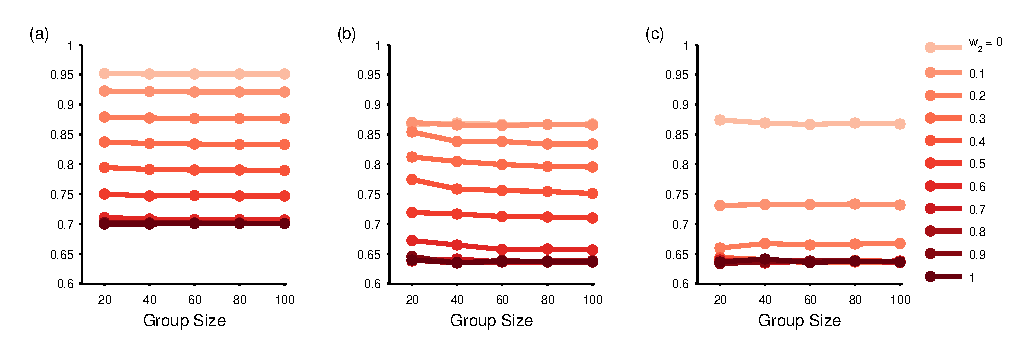
\includegraphics[width=6.83in]{group_size.pdf}
\caption{\label{groupsize} Group size does not affect the accuracy with each pair of individuals make decisions. In each panel, group size is on the horizontal axis and average accuracy is on the vertical axis. In (a) we show the average accuracy of the whole group, in (b) we show the average accuracy of the top quartile, and in (c) we show the average accuracy of the bottom quartile. Each line corresponds to a different value of $w_2$. Parameters: $N=20$, $b=1$, $r=1$, $\ell=0.1$, $w_1=0$, $w_3=1-w_2$.}
\end{figure}

\begin{figure}[ht]
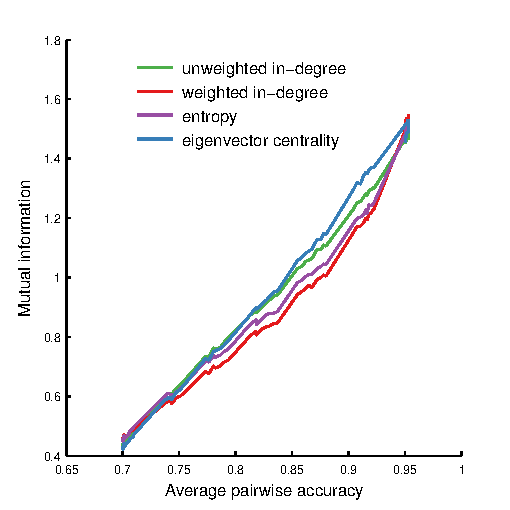
\includegraphics[width=3.4in]{mutinfo_vs_accuracy.pdf}
\caption{ }
\end{figure}

\begin{figure}[ht]
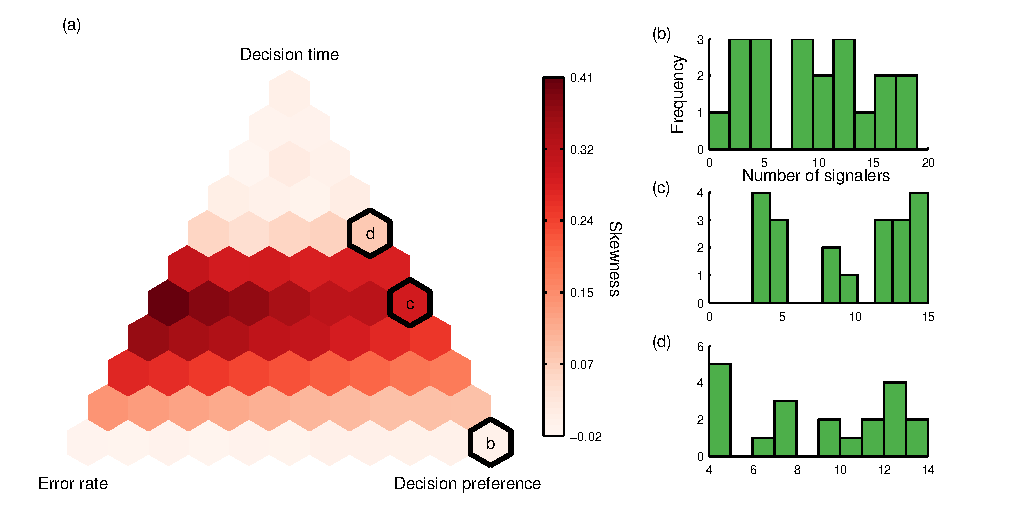
\includegraphics[width=6.83in]{skewness_histograms.pdf}
\caption{ }
\end{figure}

\begin{figure}[ht]
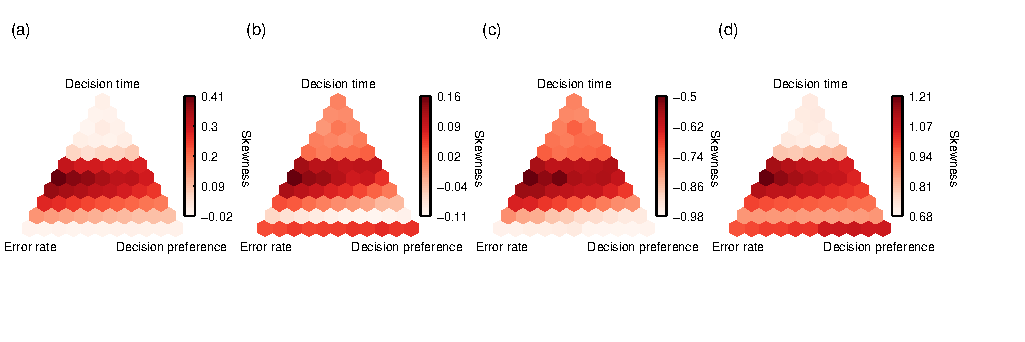
\includegraphics[width=6.83in]{multi_skewness.pdf}
\caption{\label{supp_skewness} The skewness of the consensus scores is maximized at intermediate waiting costs for every consensus measure. In each panel, the color indicates the average skewness of the consensus scores of a group using Nash thresholds, as a function of the optimization weights, $w_1$, $w_2$, $w_3$. In the lower left corner of the simplex, only error rate matters ($w_1=1$).  In the upper corner, only decision time matters ($w_2=1$).  In the lower right corner, only preference matters ($w_3=1$). In (a) consensus is given by weighted in-degree, in (b) by entropy, and in (c) by eigenvector centrality. Parameters: $N=20$, $b=1$, $r=1$, $\ell=0.1$.} 
\end{figure}

%\begin{figure}[ht]
%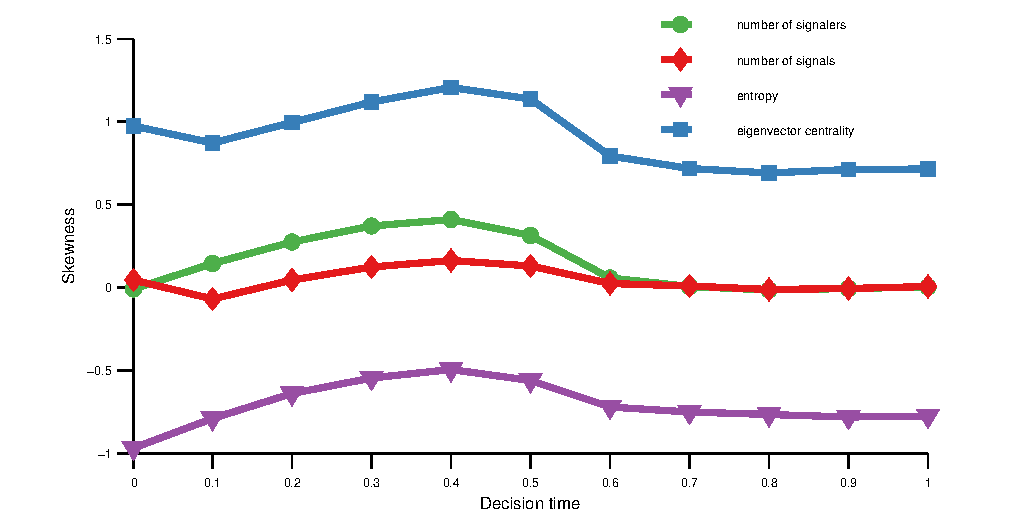
\includegraphics[width=3.4in]{skewness_max.pdf}
%\caption{ }
%\end{figure}

\pagebreak
\nocite{*}
\bibliographystyle{plain}
\bibliography{signaling_model}

\end{document}


